\chapter{ Конструкторский раздел}
\label{cha:design}
        В данном разделе будут рассмотрены описание системы, требования к функциональности ПО,
        определены способы тестирования и представлена схема алгоритма.
    \section{Описание системы}
Общая идея конвейера связана с разбиением некоторого процесса обработки объектов на независимые этапы и организацией параллельного выполнения во времени различных этапов обработки различных объектов, передвигающихся по конвейеру от одного этапа к другому.
Поэтому основой разработки конвейера является разбиение процесса на независимые этапы.

Конвейер состоит из трех лент, которые называются PreProc, Proc и PostProc. Каждый объект проходит три этапа обработки на каждой из лент. Объект представляет собой экземпляр специально созданного класса MyObject. В связи с тем, что одной из задач данной работы является проектирование ПО, реализующего конвейерную обработку (а не реализация каких-либо определенных алгоритмов), Объекты класса MyObject по сути являются абрстракцией объектов, которые обрабатывались бы в реальной конкретной системе с конвейерными вычислениями. Три ленты конвейера представляют собой три отдельных класса, каждый из которых имеет свое заранее заданное время обработки. Ленты лишь имитируют обработку объектов, приостанавливая выполнение программы на время обработки, заданное для каждой ленты. Каждая лента запускается в отдельном потоке.

В программе N объектов генерируются и помещаются в очередь первой ленты (PreProc). После того, как i-й объект (i = 1, ..., N) был обработан на первой ленте, он передается в очередь второй ленты (Proc). После обработки на второй ленте объект передается в очередь третьей ленты (PostProc). После обработки на третьей ленты объект помещается в контейнер обработанных объектов. Объект считается обработанным, если он прошел все три ленты конвейера. Эти действия выполняются для каждого из N сгенерированных объектов.

Для ленты PreProc время обработки было установлено в 50, для ленты Proc - 70, для ленты PostProc - 20.

Ниже изображена схема алгоритма обработки объектов класса MyObject (рисунок \ref{png:obj}).

        \begin{figure}[h!]
            \centering
            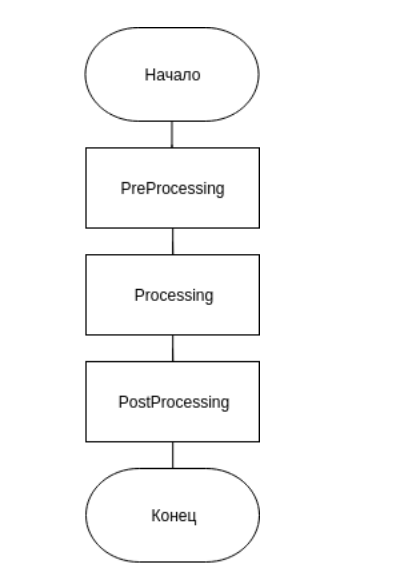
\includegraphics[scale=0.6]{obj.png}
 \caption{Алгоритм обработки объектов класса MyObject}
            \label{png:obj}
        \end{figure} 

Принцип обработки объектов на ленте PreProcessing (рисунок \ref{png:pre}).

        \begin{figure}[h!]
            \centering
            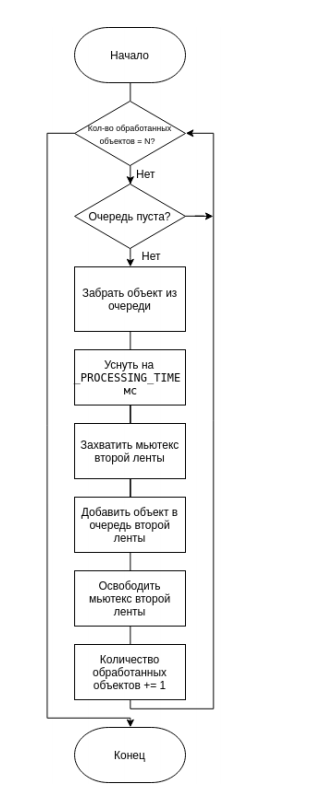
\includegraphics[scale=0.8]{pre.png}
\caption{Алгоритм обработки объектов на ленте PreProcessing}
            \label{png:pre}
        \end{figure} 

Принцип обработки объектов на ленте Processing (рисунок \ref{png:pro}).

        \begin{figure}[h!]
            \centering
            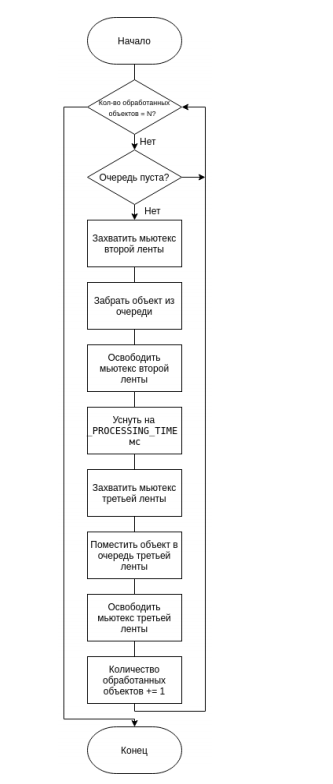
\includegraphics[scale=0.85]{pro.png}
\caption{Алгоритм обработки объектов на ленте Processing}
            \label{png:pro}
        \end{figure} 

Принцип обработки объектов на ленте PostProcessing (рисунок \ref{png:post}).

        \begin{figure}[h!]
            \centering
            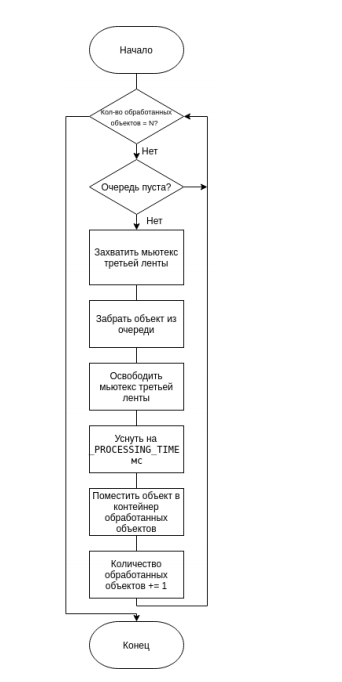
\includegraphics[scale=0.85]{post.png}
\caption{Алгоритм обработки объектов на ленте PostProcessing}
            \label{png:post}
        \end{figure} 

    \section{Требования к функциональности ПО}
        В данной работе требуется обеспечить следующую минимальную функциональность консольного приложения:
        \begin{enumerate}
            \item предоставить возможность ввода количества генерируемых элементов в системе;
            \item обеспечить вывод времени получения и отправки элемента конвейера.
        \end{enumerate}
	Кроме этого, должен быть создан log-file, куда должно быть записано общее время работы конвейера.

    \section{Тесты}
        Тестирование ПО будет проводиться методом чёрного ящика. 


    \section{Вывод}
        В данном разделе были рассмотрены схема алгоритмов 
        обработки элементов линии конвейера и
        описаны требования к функциональности ПО.
        

\newpage